\documentclass[12pt]{beamer}

% Turn off the ugly navigation symbols.
\setbeamertemplate{navigation symbols}{}

% Margins and whatnot.
\setbeamersize{text margin left=2em,text margin right=2em}

\usepackage{fontspec}
\defaultfontfeatures{Mapping=tex-text} % enable -- / --- / `` / ''
\usefonttheme{serif}
\setmainfont{Helvetica}
\setsansfont{Oswald}
\setmonofont{Courier}

\definecolor{verydarkgrey}{HTML}{001112}
\definecolor{darkblue}{HTML}{232747}
\definecolor{grey}{HTML}{777777}

\setbeamerfont{frametitle}{size=\Large}
\setbeamercolor{frametitle}{fg=black}
\setbeamercolor{titleline}{bg=black}
\setbeamercolor{title}{fg=black}
\setbeamercolor*{date in head/foot}{fg=grey}
\setbeamercolor{item}{fg=black}
\setbeamerfont{item}{series=\bfseries}
% Never used, but this is nice.
\setbeamertemplate{itemize subitem}{--}
\setbeamerfont{itemize/enumerate subbody}{size=\small}

% \useoutertheme{new}

\makeatletter
\usepackage{dashrule}
\defbeamertemplate*{frametitle}{mine}[1][left]
{
  % Increase width of title box
  \@tempdima=\textwidth%
  \advance\@tempdima by\beamer@leftmargin%
  \advance\@tempdima by\beamer@rightmargin%
  %
  \begin{beamercolorbox}[sep=0.3cm,#1,wd=\the\@tempdima]{frametitle}
    \usebeamerfont{frametitle}%
    \vbox{}\vskip-1ex\vspace{.5ex}
    \strut\hspace{2ex}\sf\insertframetitle\strut\par%
    \vskip-1.5ex%
    \hspace{\fill}%
    %\hdashrule{\textwidth}{.075ex}{.075ex .2ex}%
    \color{black}{\rule{\textwidth}{.075ex}}%
    \hspace{\fill}%
    \par\nointerlineskip \vspace{\baselineskip}
  \end{beamercolorbox}%
  \nointerlineskip%
  \vspace{-3.5ex}
}

% \defbeamertemplate*{footline}{}
% {
%   \hbox{%
%   \begin{beamercolorbox}[wd=.8\paperwidth]{section in head/foot}%
%   \end{beamercolorbox}%
%   \begin{beamercolorbox}[wd=.2\paperwidth,ht=2.25ex,dp=1ex,right]{date in head/foot}%
%     \insertframenumber{} / \inserttotalframenumber\hspace*{2ex} 
%   \end{beamercolorbox}}%
%   \vskip0pt%
% }
\makeatother


\usepackage{fancyvrb}
\usepackage{fancyvrb}
\usepackage{xcolor}
\usepackage{relsize}
\newcommand{\code}{\texttt}
\usepackage{url}
\newcommand{\Rstar}{R$^*$}

\newcommand{\wikipic}[1]{%
\begin{center}%
\includegraphics[width=.8\textwidth]{figure/simple_models_#1}%
\end{center}}
\newcommand{\wikipich}[1]{%
\begin{center}%
\includegraphics[height=.8\textheight]{figure/simple_models_#1}%
\end{center}}
\newcommand{\subt}[1]{{~~~\normalsize (#1)}}

\begin{document}

\begin{frame}
  \thispagestyle{empty}
  \begin{center}
    \sf
    {\Huge Competition Kernels}\\[2ex]
    % {\footnotesize {}}\\[1.5em]
    {\large Rich FitzJohn}\\[3em]
    {Lab meeting, 2014-05-13}
  \end{center}
\end{frame}

% plant_competition.jpg
%   http://www.mnartists.org/uploads/users/user_19614/753e6ea77020019fc17a27512c71a41d/753e6ea77020019fc17a27512c71a41d.jpg
%
% animal_competition.jpg
%  http://fabuloustraveling.com/wp-content/uploads/2013/06/133.jpg
\begin{frame}
  \begin{center}
    \includegraphics<1>[height=\textheight]{pics/plant_competition} 
    \includegraphics<2>[width=\textwidth]{pics/animal_competition}
  \end{center}
\end{frame}

\begin{frame}[t]{Competition and coexistance}
  \begin{center}
    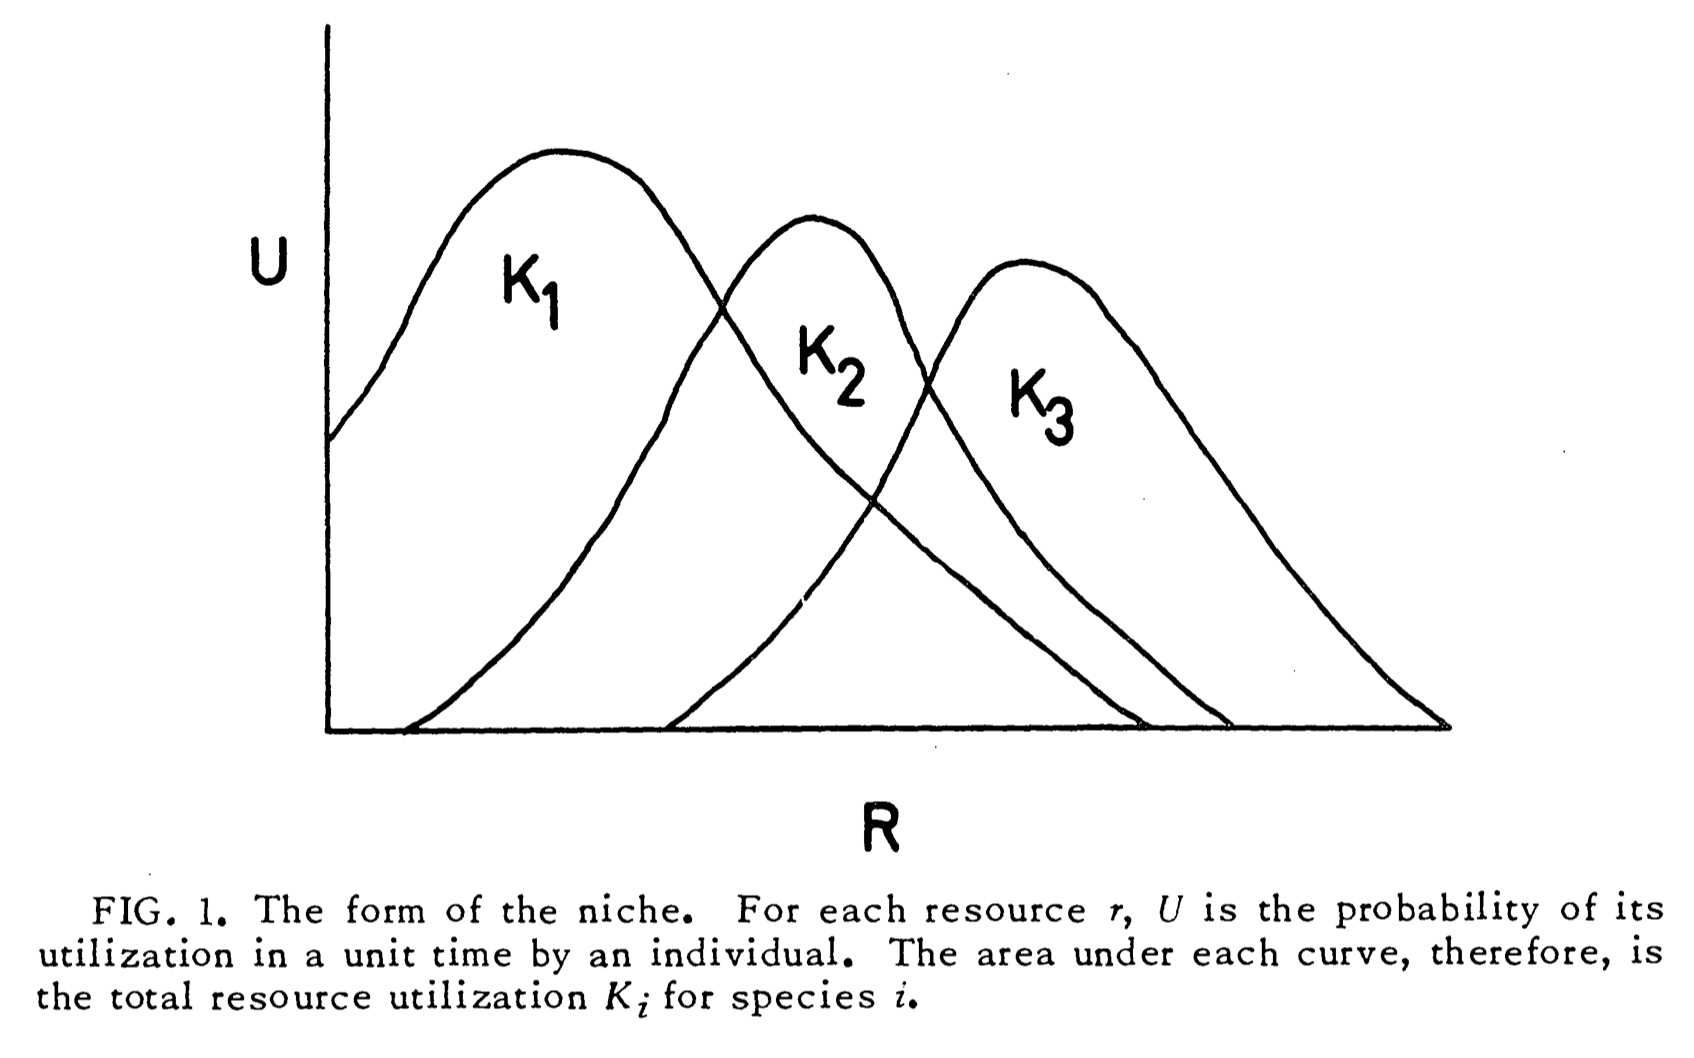
\includegraphics[width=.8\textwidth]{pics/limiting_similarity.png}
    
    \small ``Limiting similarity'' --- MacArthur and Levins 1967
  \end{center}
\end{frame}

% http://geology.gsapubs.org/content/30/1/15/F1.expansion.html
\begin{frame}[t]{Competition and coexistance}
  \begin{center}
    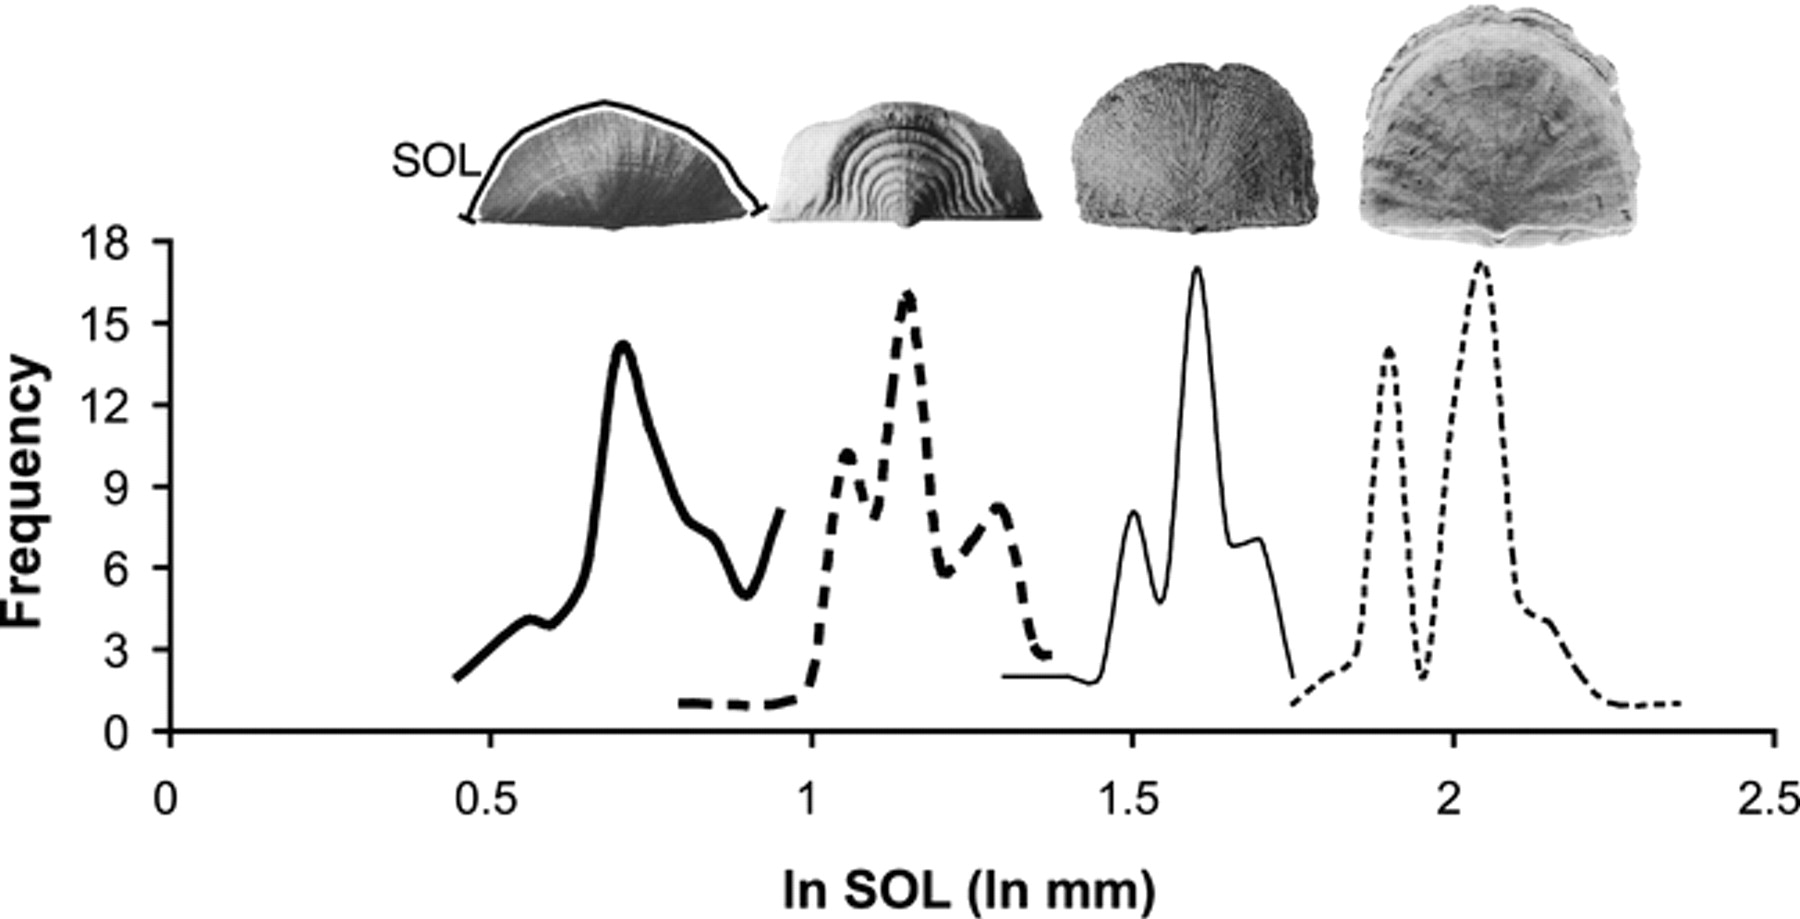
\includegraphics[width=.8\textwidth]{pics/hermoyian-2002.jpg}
    
    Hermoyian et al. 2002
  \end{center}
\end{frame}

\begin{frame}[t]{Character displacement}
  \begin{center}
    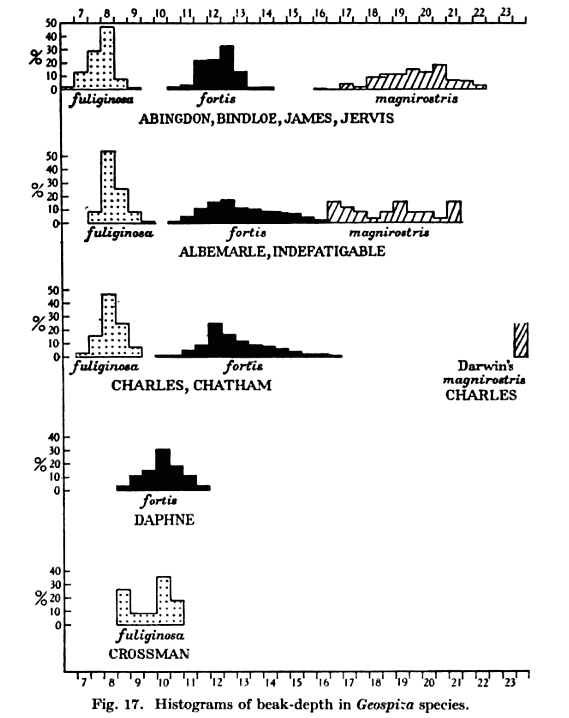
\includegraphics[height=.8\textheight]{pics/finches}

    \small Lack 1947
  \end{center}
\end{frame}

\begin{frame}[t]{Aims:~~~proximate aim}
 Measure the shape of competition with respect to traits.
 \begin{itemize}
 \item ``Competition kernel''
 \item In models mostly, but possibly in biological data
 \item Qualitatively: symmetric, asymmetric?
 \item Variation with abundance: linear, saturating, accelerating?
 \item In models with known kernels
 \end{itemize}
\end{frame}

\begin{frame}[t]{Aims:~~~ultimate aim \& implications}
 \begin{itemize}
 \item How reasonable are commonly used
   functions?
   \begin{itemize}
   \item Key ingredient for models of coexistence, population
     dynamics, evolution of traits, character displacement, etc.
   \end{itemize}
 \item What are experiments that measure competition really
   measuring?
 \item Coexistence question: do different competition kernels lead
   to different patterns of coexistence?
   \begin{itemize}
   \item Leimar et al. approach answered some of this
   \item Interaction with ``carrying capacity'' important
   \item Competition appears not sufficient information to determine
     patterns of coexistence.
   \end{itemize}
 \item Which types of factors generate symmetry/asymmetry in
   competition?
 \end{itemize}
\end{frame}


\begin{frame}[t]{Approach}
  \begin{itemize}
  \item Think about what competition \emph{means}
  \item Start with models with ``explicit competition'' and recover
    this
    \begin{itemize}
    \item Models where the competition function is baked directly into
      the model - if we know what it is already, should be able to
      recover it as a test case.
    \end{itemize}
  \item Next, relatively simple models with ``implicit competition''.
    \begin{itemize}
    \item Models where competition \emph{emerges}, e.g., via shared
      resource use.
    \end{itemize}
  \item Complicated mechanistic models with implicit competition based
    on things we know about species
    \begin{itemize}
    \item Starting with Daniel's vegetation model.
    \end{itemize}
  \end{itemize}
\end{frame}

\begin{frame}[t]{Simple models}
  \begin{itemize}
  \item Explicit competition:
      \begin{itemize}
      \item Dieckmann and Doebeli 1999: symmetric Gaussian competition\\
        (speciation by disruptive selection)
      \item Kisdi 1999: Asymmetric (logistic) competition\\
        (evolutionary arms races)
      \end{itemize}
  \item Implicit competition:
      \begin{itemize}
      \item Tilman 1982 (\& various) \Rstar model\\
        Shared use of resources
      \end{itemize}
  \item Mechanistic competition:
    \begin{itemize}
    \item Falster 2010/2014\\
      Forest stand with competition for light
    \end{itemize}
  \end{itemize}
\end{frame}

\begin{frame}[t]{Dieckmann and Doebeli 1999 \subt{Gaussian}}
  \begin{itemize}
    \item Key features:
      \begin{itemize}
      \item Competition reduces a species carrying capacity via a
        Gaussian function, and is \textbf{symmetric} (e.g., similar
        species compete more strongly than dissimilar species).
      \item Species effects are linear with respect to density
      \item Carrying capacity is also Gaussian
      \end{itemize}
    \item Other similar models: Doebeli and Dieckmann (2010; Am Nat),
      Case and Taper (2000; Am Nat) / Goldberg and Lande (2010; Am
      Nat), Leimar et al. (2013; J Theor Biol)
      \begin{itemize}
      \item some of these have competition affecting growth rate,
        rather than carrying capacity
      \end{itemize}
    \item Doebeli and Ispolatov (2013; Math Biol) argue these are
      very general, even out to models where competition is really
      asymmetric.
  \end{itemize}
\end{frame}

\begin{frame}[t]{Gaussian competition \subt{Dieckmann and Doebeli 1999}}
  \only<1>{\wikipic{dieckmann__dd_competition_true}}
  \only<2>{\wikipic{dieckmann__dd_carrying_capacity}}
\end{frame}

\begin{frame}[t]{Gaussian competition \subt{Dieckmann and Doebeli 1999}}
  Fitness:

  \begin{center}
    \begin{displaymath}
      w(x^\prime, x, y) = 
      r\left(1 - \frac{\sum_{i=1}^N
          N_i \, {\color{red}\exp\left(-\frac{(x^\prime-x_i)^2}{2\sigma_C^2}\right)}}
        {K_0 \exp \left(-\frac{{x^\prime}^2}{2\sigma_K^2}\right)}
      \right)
    \end{displaymath}
  \end{center}
\end{frame}

\begin{frame}[t]{Gaussian competition \subt{Dieckmann and Doebeli 1999}}
  Fitness:
  \wikipic{dieckmann__dd_fitness_landscape}
\end{frame}

\begin{frame}[t]{Kisdi 1999 \subt{Asymmetric}}
  \begin{itemize}
    \item Key features:
      \begin{itemize}
      \item Competition reduces a species growth rate via a logistic
        function, and is \textbf{asymmetric} (e.g., larger species are
        competitively superior)
      \item Species effects are linear with respect to density
      \item Carrying capacity is linear (in opposite direction to
        competitive hierarchy) or Gaussian.
      \end{itemize}
    \item Similar models include Geritz et al. (1999; Theor Pop Biol)
      for seed size.
    \item Less common than symmetric models
  \end{itemize}
\end{frame}

\begin{frame}[t]{Asymmetric \subt{Kisdi 1999}}
  \wikipic{kisdi__k_competition_felt}
\end{frame}

\begin{frame}[t]{Asymmetric \subt{Kisdi 1999}}
  \begin{itemize}
  \item Note that this is competition \textbf{felt}
  \item Species with low trait values have their growth suppressed by
    bigger species, but that is compensated by a higher intrinsic
    growth rate (I think mathematically similar to the carrying
    capacity?)
  \item In contrast, competition exerted:
  \end{itemize}
\end{frame}

\begin{frame}[t]{Asymmetric \subt{Kisdi 1999}}
  \wikipic{kisdi__k_competition_true}
\end{frame}

\begin{frame}[t]{Asymmetric \subt{Kisdi 1999}}
  Fitness:
  \begin{displaymath}
      w(x^\prime, x, y) = 
      \rho(x) - 
        \sum_{i=1}^N N_i \,
        {\color{red}\alpha(x_i - x_j)}
  \end{displaymath}
  \begin{displaymath}
      w(x^\prime, x, y) = 
      \rho(x) - 
        \sum_{i=1}^N N_i \,
        {\color{red}c\left(
            1 - \frac{1}{1 + \exp(-k(x_i - x_j))}
            \right)}
  \end{displaymath}
\end{frame}

\begin{frame}[t]{Asymmetric \subt{Kisdi 1999}}
  Fitness:
  \only<1>{\wikipic{kisdi__k_fitness_landscape}}
  \only<2>{\wikipic{kisdi__k_fitness_landscape_detail}}
\end{frame}

\begin{frame}
  \large
  If all we can use is the fitness function, how do we infer the shape of
  competition?

  \pause
  \vspace{1em}
  Sensitivity of fitness to resident density

  \begin{displaymath}
    \left. \frac{d w_i}{d N_j} \right|_{N_i = 0, N_j = \hat N_j}
  \end{displaymath}

  \pause
  \vspace{1em}
  If increasing density of resident decreases invader fitness, the
  invader is being competed against by the resident.
\end{frame}

\begin{frame}[t]{Fitness Jacobian}
  \only<1>{\wikipic{dieckmann__dd_mutant_1}}
  \only<2>{\wikipic{dieckmann__dd_mutant_2}}
  \only<3>{\wikipic{dieckmann__dd_mutant_2_slope}}
  \only<4>{\wikipic{dieckmann__dd_derivative}}
  \only<5>{\wikipic{dieckmann__dd_derivative_scaled}}
  \only<6>{\wikipic{kisdi__k_derivative}}
\end{frame}

\begin{frame}[t]{Tilman 1982\subt{R star}}
  \begin{itemize}
  \item Key features:
    \begin{itemize}
    \item No explicit competition kernel, no explicit carrying
      capacity
    \item Species consume shared resources at some rate and convert
      them into offspring
    \item Externally specified rate of resource regeneration
    \item For k resources, up to k species can coexist
    \item Species ``draw down'' resources to their \Rstar; species
      with higher requirements die.
    \end{itemize}
  \item Terrifying literature of variants and tweaks
  \item Probably the simplest possible shared resource model
  \item Considering single resource case here (one winner)
  \end{itemize}
\end{frame}

\begin{frame}[t]{R star \subt{Tilman 1982}}
  Fitness, with respect to parameter affecting rate of conversion to
  new offspring (bigger K, more required)
  \wikipic{rstar_1__r1_fitness_landscape_K}
\end{frame}

\begin{frame}[t]{R star \subt{Tilman 1982}}
  As a function of resident density
  \wikipic{rstar_1__r1_mutant_1}
\end{frame}

\begin{frame}[t]{R star \subt{Tilman 1982}}
  Invader fitness sensitivity to resident:
  \only<1>{\wikipic{rstar_1__r1_mutant_1_slope}}
  \only<2>{\wikipic{rstar_1__r1_derivative}}
\end{frame}

\begin{frame}[t]{R star \subt{Tilman 1982}}
  \begin{itemize}
  \item This is confusing:
    \begin{itemize}
    \item Species with low K values who will replace the resident are
      most strongly competed against by the resident.
    \item But these species also have the highest \textbf{potential}
      fitness
    \end{itemize}
  \end{itemize}
\end{frame}

\begin{frame}[t]{R star \subt{Tilman 1982}}
  Fitness in empty environment:
  \wikipic{rstar_1__r1_fitness_empty}
\end{frame}

\begin{frame}[t]{R star \subt{Tilman 1982}}
  Scale $w$ to get $w / w_{max}$ and take derivative of \emph{that}:
  \wikipic{rstar_1__r1_derivative_scaled}
\end{frame}

\begin{frame}[t]{R star \subt{Tilman 1982}}
  Competition stronger, and more trait dependent under low resources
  \wikipic{rstar_1__r1_derivative_scaled_S}
\end{frame}

% Hmm - looks like the point where competition becomes non-unimodal in
% density is at the resident density equilibrium.  That's interesting.
\begin{frame}[t]{R star \subt{Tilman 1982}}
  Nonlinear competition with density
  \only<1>{\wikipic{rstar_1__r1_mutant_1_slope}}
  \only<2>{\wikipic{rstar_1__r1_fitness_varying}}
  \only<3>{\wikipic{rstar_1__r1_fitness_varying_scaled}}
  \only<4>{\wikipic{rstar_1__r1_derivative_varying_scaled}}
  \only<5>{\wikipic{rstar_1__r1_derivative_varying_scaled_twice}}
  \only<6>{\wikipic{rstar_1__r1_derivative_scaled_twice_image}}
  \only<7>{\wikipich{rstar_1__r1_derivative_scaled_twice_3d}}
\end{frame}

\begin{frame}[t]{Where next?}
  \begin{itemize}
  \item Is this a sensible measure?  Seems very sensitive to scaling,
    and negative ``potential fitness'' causes real problems.
  \item R star 2 resource model (really weird)
  \item Falster 2010/2014 (really, really weird)
  \item What do these mean for Lotka-Volterra models?
  \item Age structured models
  \item Multiple residents and the other linear assumption
  \item Connection with empirical literature - \textbf{curvature} of
    density is used there.
  \end{itemize}
\end{frame}

\end{document}

%%% Local Variables: 
%%% mode: latex
%%% TeX-PDF-mode: t
%%% TeX-engine: xetex
%%% End: 

%  LocalWords:  Tilman Dieckmann Lande Leimar Theor Ispolatov Geritz
%  LocalWords:  dieckmann kisdi Jacobian rstar Lotka Volterra
